\documentclass[11pt]{article}
\usepackage[margin=1in]{geometry}
\usepackage{amsmath,amssymb,amsthm}
\usepackage{graphicx}
\usepackage[hidelinks]{hyperref}

\newtheorem{theorem}{Theorem}
\newtheorem{lemma}{Lemma}
\newtheorem{corollary}{Corollary}

\newcommand{\B}{\mathbb{B}}
\newcommand{\R}{\mathbb{R}}
\newcommand{\id}{\operatorname{id}}
\newcommand{\sgn}{\operatorname{sgn}}
\newcommand{\supp}{\operatorname{supp}}

\title{Surjective isometries of the real \(L^1[0,1]\) ball are extremal}
\author{Run \texttt{fa\_banach\_001}, lane 8}
\date{2026-06-19}

\begin{document}
\maketitle

\paragraph{Status.}
Candidate full solution, likely valid pending human review. The proof is for
real \(L^1\). The complex case should be formulated separately using real
supporting hyperplanes and phase functions.

\paragraph{Source problem.}
Bargetz, Dymond, and Pirk \cite{BDP} prove that surjective isometries of the
closed unit ball are extremal for many classical Banach spaces. They explicitly
single out \(L^1[0,1]\) as the remaining classical case not covered by their
Theorem 1.1 and write that they do not know whether surjective isometries of
the closed unit ball of \(L^1[0,1]\) are extremal.

\begin{center}

\includegraphics[width=\linewidth]{figures/open_problem_crop.png}
\end{center}

The source paper's nonlinear proof under hypothesis (i) uses the closed convex
hull of almost exposed points:

\begin{center}
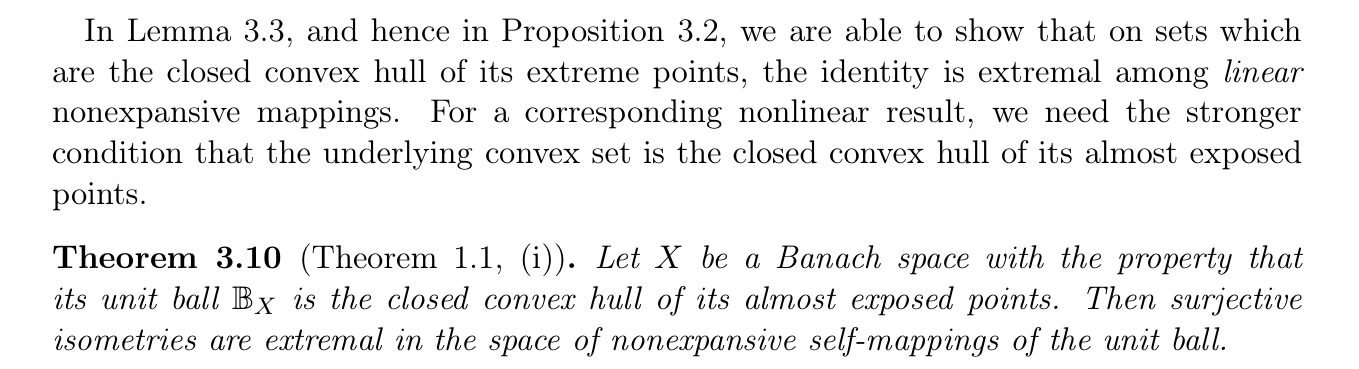
\includegraphics[width=\linewidth]{figures/method_condition_crop.png}
\end{center}

The proof below does not use almost exposed points. It uses the full family of
norming faces of the \(L^1\)-ball instead.

\section*{Proof Intuition}

Suppose
\[
   \id=(1-\lambda)F+\lambda G,\qquad 0<\lambda<1,
\]
where \(F\) and \(G\) are nonexpansive self-maps of the \(L^1\)-unit ball. As
observed in \cite{BDP}, \(F\) and \(G\) must themselves be isometries. The
extra \(L^1\)-specific observation is that every norming functional of a unit
vector \(f\) must also norm \(F(f)\) and \(G(f)\). Hence \(F(f)\) and \(G(f)\)
are trapped in the same norming face as \(f\): they have the same sign as
\(f\) and no mass outside the support of \(f\).

This face preservation is very rigid when combined with isometry. A signed
normalized indicator of a set \(A\) cannot be moved inside \(A\): comparing
distances to the signed normalized indicators of all subsets \(B\subset A\)
forces its image to put at least the normalized Lebesgue mass on every
measurable subset of \(A\), hence exactly that mass. The same argument then
fixes signed simple unit vectors, and density fixes the whole unit sphere.

It remains to rule out movement inside the ball. Once the sphere is fixed,
distances from an interior point to all signed normalized indicators are
preserved. On small enough measurable pieces these distances read off the
integrals of the positive and negative parts of the point. Atomlessness lets us
make those pieces arbitrarily small, so the point itself is recovered.

\section*{Statement}

Let \((\Omega,\Sigma,\mu)\) be an atomless probability space and put
\(X=L^1(\mu;\R)\). Let \(\B_X\) be the closed unit ball of \(X\), and let
\(\mathcal M\) be the convex set of all nonexpansive maps
\(\B_X\to\B_X\).

\begin{theorem}
The identity map on \(\B_X\) is an extreme point of \(\mathcal M\). In
particular, the identity map on the closed unit ball of real \(L^1[0,1]\) is
extremal among nonexpansive self-maps.
\end{theorem}

\begin{corollary}
Every surjective isometry of the closed unit ball of real \(L^1[0,1]\) is
extremal among nonexpansive self-maps of that ball.
\end{corollary}

\begin{proof}
The corollary follows from the theorem and Lemma 3.1 of \cite{BDP}, which
reduces extremality of surjective isometries of a convex body with nonempty
interior to extremality of the identity by conjugating with the inverse
isometry. Thus it suffices to prove the theorem.
\end{proof}

\section*{Proof of the theorem}

Assume
\[
   \id=(1-\lambda)F+\lambda G,\qquad 0<\lambda<1,
\]
with \(F,G\in\mathcal M\). We prove \(F=G=\id\).

First, \(F\) and \(G\) are isometries. Indeed, for \(x,y\in\B_X\),
\[
\begin{aligned}
\|x-y\|_1
&=\|(1-\lambda)(F(x)-F(y))+\lambda(G(x)-G(y))\|_1\\
&\le (1-\lambda)\|F(x)-F(y)\|_1+\lambda\|G(x)-G(y)\|_1\\
&\le \|x-y\|_1.
\end{aligned}
\]
Both inequalities must be equalities, so
\(\|F(x)-F(y)\|_1=\|G(x)-G(y)\|_1=\|x-y\|_1\).

\begin{lemma}[Face preservation on the sphere]
Let \(T\) denote either \(F\) or \(G\). If \(f\in X\) and \(\|f\|_1=1\), put
\[
   A=\{\omega:f(\omega)\ne0\},\qquad s=\sgn f .
\]
Then
\[
   T(f)=s q
\]
for some \(q\ge0\) supported in \(A\) with \(\int_A q\,d\mu=1\).
\end{lemma}

\begin{proof}
Let \(\varphi\in L^\infty(\mu)\) be any norming functional for \(f\), so
\(\|\varphi\|_\infty=1\) and \(\int\varphi f\,d\mu=1\). Applying \(\varphi\)
to the decomposition of \(f\) gives
\[
   1=(1-\lambda)\int\varphi F(f)\,d\mu
      +\lambda\int\varphi G(f)\,d\mu .
\]
Both integrals are at most \(1\), since \(F(f),G(f)\in\B_X\). Hence both are
equal to \(1\). In particular, \(T(f)\) lies in every supporting hyperplane of
\(\B_X\) at \(f\).

The normalized supporting functionals at \(f\) are precisely those
\(\varphi\in L^\infty\) with \(\|\varphi\|_\infty=1\) and \(\varphi=s\) a.e.
on \(A\). Taking the particular functional \(s1_A\), equality
\(\int_A sT(f)\,d\mu=1\) and \(\|T(f)\|_1=1\) force
\[
   T(f)=0\ {\rm a.e.\ on}\ \Omega\setminus A,\qquad sT(f)=|T(f)|\ {\rm a.e.}
\]
Thus \(T(f)=sq\), where \(q\ge0\), \(q\) is supported in \(A\), and
\(\int_A q\,d\mu=1\).
\end{proof}

\begin{lemma}[The isometries fix the unit sphere]
Let \(T\) denote either \(F\) or \(G\). Then \(T(f)=f\) for every
\(f\in X\) with \(\|f\|_1=1\).
\end{lemma}

\begin{proof}
For a measurable \(A\) with \(\mu(A)>0\) and \(\varepsilon\in\{-1,1\}\), write
\[
   u_A^\varepsilon=\varepsilon\,\frac{1_A}{\mu(A)} .
\]
By the previous lemma,
\[
   T(u_A^\varepsilon)=\varepsilon q_A
\]
where \(q_A\ge0\), \(q_A\) is supported in \(A\), and \(\int_A q_A\,d\mu=1\).
If \(B\subset A\) has positive measure, then
\[
   \|u_A^\varepsilon-u_B^\varepsilon\|_1
      =2\left(1-\frac{\mu(B)}{\mu(A)}\right).
\]
Since \(T\) is an isometry and \(T(u_B^\varepsilon)\) is supported in \(B\)
with sign \(\varepsilon\), we also have
\[
\begin{aligned}
2\left(1-\frac{\mu(B)}{\mu(A)}\right)
&=\|T(u_A^\varepsilon)-T(u_B^\varepsilon)\|_1\\
&\ge 2\left(1-\int_B q_A\,d\mu\right).
\end{aligned}
\]
Thus \(\int_B q_A\,d\mu\ge \mu(B)/\mu(A)\) for every \(B\subset A\). Since
both measures have total mass \(1\) on \(A\), \(q_A=\mu(A)^{-1}1_A\) a.e.
Therefore \(T\) fixes every signed normalized indicator \(u_A^\varepsilon\).

Now let \(f\) be a signed simple unit vector,
\[
   f=\sum_{i=1}^n \varepsilon_i\alpha_i\,\frac{1_{A_i}}{\mu(A_i)},
\]
where the \(A_i\) are pairwise disjoint measurable sets of positive measure,
\(\varepsilon_i\in\{-1,1\}\), \(\alpha_i>0\), and \(\sum_i\alpha_i=1\). By
face preservation,
\[
   T(f)=s q,\qquad s=\sgn f,
\]
where \(q\ge0\), \(q\) is supported in \(\bigcup_i A_i\), and \(\int q=1\).
For \(u_i=\varepsilon_i1_{A_i}/\mu(A_i)\), already fixed by \(T\),
\[
   \|f-u_i\|_1=2(1-\alpha_i).
\]
The same lower-bound argument gives \(\int_{A_i}q\,d\mu\ge\alpha_i\). Summing
over \(i\) yields equality for every \(i\). If \(B\subset A_i\), then
\[
   \left\|f-\varepsilon_i\frac{1_B}{\mu(B)}\right\|_1
      =2\left(1-\alpha_i\frac{\mu(B)}{\mu(A_i)}\right),
\]
and the lower-bound argument gives
\[
   \int_B q\,d\mu\ge \alpha_i\frac{\mu(B)}{\mu(A_i)} .
\]
Since \(\int_{A_i}q\,d\mu=\alpha_i\), it follows that
\(q=\alpha_i\mu(A_i)^{-1}\) a.e. on \(A_i\). Hence \(T(f)=f\).

Signed simple unit vectors are dense in the unit sphere of \(L^1(\mu)\), and
\(T\) is continuous because it is an isometry. Therefore \(T\) fixes the whole
unit sphere.
\end{proof}

\begin{lemma}[Fixing the sphere fixes the ball]
Let \(T:\B_X\to\B_X\) be an isometry that fixes every point of the unit sphere
of \(X=L^1(\mu;\R)\), where \(\mu\) is atomless. Then \(T=\id\).
\end{lemma}

\begin{proof}
First \(T(0)=0\). If \(z=T(0)\ne0\), choose a measurable set \(B\) of positive
measure on which \(z\) has one sign and \(\int_B |z|\,d\mu>0\). Taking the
oppositely signed normalized indicator \(u\) on \(B\), which is fixed by \(T\),
we get
\[
   1=\|0-u\|_1=\|T(0)-T(u)\|_1=\|z-u\|_1=1+\int_B|z|\,d\mu+\int_{\Omega\setminus B}|z|\,d\mu>1,
\]
a contradiction.

Let \(x\in\B_X\) and set \(z=T(x)\). Since \(T(0)=0\), \(\|z\|_1=\|x\|_1\).
For every measurable \(B\) with \(\mu(B)>0\) and every
\(\varepsilon\in\{-1,1\}\), the signed normalized indicator
\(u_B^\varepsilon=\varepsilon1_B/\mu(B)\) is fixed. Therefore
\[
   \|x-u_B^\varepsilon\|_1=\|z-u_B^\varepsilon\|_1 .
\]
For any \(w\in L^1(\mu)\),
\[
   \|w-u_B^\varepsilon\|_1
   =\|w\|_1+1-2\int_B
      \min\left((\varepsilon w)_+,\frac1{\mu(B)}\right)\,d\mu .
\]
Because \(\|x\|_1=\|z\|_1\), we get
\[
   \int_B \min\left((\varepsilon x)_+,\frac1{\mu(B)}\right)\,d\mu
   =
   \int_B \min\left((\varepsilon z)_+,\frac1{\mu(B)}\right)\,d\mu
\]
for every \(B\) and every sign \(\varepsilon\).

Fix \(\varepsilon\) and \(M>0\). Let
\[
   E_M=\{(\varepsilon x)_+\le M\}\cap\{(\varepsilon z)_+\le M\}.
\]
If \(C\subset E_M\), atomlessness and finiteness of \(\mu\) allow us to
partition \(C\) into finitely many measurable pieces \(C_j\) with
\(\mu(C_j)<1/M\), ignoring null pieces. On each \(C_j\) the truncation level
\(1/\mu(C_j)\) is larger than \(M\), so the displayed equality gives
\[
   \int_{C_j}(\varepsilon x)_+\,d\mu
   =
   \int_{C_j}(\varepsilon z)_+\,d\mu .
\]
Summing over \(j\) gives equality of the integrals over \(C\). Since this holds
for every \(C\subset E_M\), the two functions \((\varepsilon x)_+\) and
\((\varepsilon z)_+\) agree a.e. on \(E_M\). Letting \(M\to\infty\), they
agree a.e. on \(\Omega\). Applying this for \(\varepsilon=1\) and
\(\varepsilon=-1\) gives \(x^+=z^+\) and \(x^-=z^-\). Hence \(x=z\).
\end{proof}

Applying the last two lemmas to \(F\) and \(G\), both maps fix the unit sphere
and hence the whole closed unit ball. Thus \(F=G=\id\), so the identity is
extremal.

\section*{Verification and novelty check}

The proof is analytic and self-contained except for two source-paper facts:
the reduction from surjective isometries to the identity, and the elementary
observation that summands in a convex decomposition of an isometry are
isometries. Both are reproduced or cited above.

Local index search found no existing full packet for arXiv:2409.04292. The
only exact run hit was the preceding partial packet
\texttt{2409.04292\_l1\_almost\_exposed\_atoms}, now superseded by this
candidate full solution. Web searches on 2026-06-19 for the exact
\(L^1[0,1]\) extremality phrases and related ``extreme nonexpansive mappings
L1'' terms found the source paper but no later answer. This is not a proof of
novelty, but it supports treating the packet as a candidate new solution.

Human review should focus on the two rigidity lemmas: first, the domination
argument for signed normalized indicators; second, the local recovery of
interior points from distances to signed normalized indicators.

\begin{thebibliography}{9}
\bibitem{BDP}
Christian Bargetz, Michael Dymond, and Katriin Pirk.
\newblock On extremal nonexpansive mappings.
\newblock arXiv:2409.04292, 2024.
\newblock \url{https://arxiv.org/abs/2409.04292}.
\end{thebibliography}

\end{document}
